\documentclass[12pt,a4paper]{article}

\usepackage[in, plain]{fullpage}
\usepackage{array}
%\usepackage{../../../pas-math}
\usepackage{../../../moncours2}

%\makeatletter
%\renewcommand*{\@seccntformat}[1]{\csname the#1\endcsname\hspace{0.1cm}}
%\makeatother


%\author{Olivier FINOT}
\date{}
\title{\textcircled{{\normalsize{10}}} Parallélogrammes particuliers}

\graphicspath{{./img/}}
%\rfoot{Page \thepage}
\begin{document}
	\maketitle



\begin{myobj}
	\begin{itemize}
		
		\item Construire le symétrique d’un point ou d'une figure par rapport à une droite à la main où à l’aide d’un logiciel;
		\item Construire le symétrique d’un point ou d'une figure par rapport à un point, à la main où à l’aide d’un logiciel;
		\item Utiliser les propriétés de la symétrie axiale ou centrale;
		\item Identifier des symétries dans des figures.		
	\end{itemize}
\end{myobj}

\begin{mycomp}
	\begin{itemize}
		\item \kw{Chercher (Ch2)} :  s’engager    dans    une    démarche    scientifique, observer, questionner, manipuler, expérimenter (sur une feuille de papier, avec des objets, à l’aide de logiciels), émettre des hypothèses, chercher des exemples ou des contre-exemples, simplifier ou particulariser une situation, émettre une conjecture ;
		\item \kw{Raisonner (Ra3)} :  démontrer : utiliser un raisonnement logique et des règles établies (propriétés, théorèmes, formules) pour parvenir à une conclusion ;
		\item \kw{Communiquer (Co2)} :  expliquer à l’oral ou à l’écrit (sa démarche, son raisonnement, un calcul, un protocole   de   construction   géométrique, un algorithme), comprendre les explications d’un autre et argumenter dans l’échange ; 
		
	\end{itemize}
\end{mycomp}




\section{Le parallélogramme}

%\begin{mydef}
	$a$ et $b$ sont deux nombres ($b$ $\neq$ 0).\pause Le \kw{quotient} de $a$ par $b$ se note $a \div b$ ou $\dfrac{a}{b}$, en écriture fractionnaire.\pause
\end{mydef}

\begin{myex}
	%\begin{itemize}
		%\item 
		Le quotient de 5 par 4 est $\dfrac{5}{4}$, c'est le nombre qui multiplié par 4 donne 5. \pause
		\begin{equation*}
			\dfrac{5}{4} \times 4 = 5
		\end{equation*}

		%\item Le quotient de 2 par 3 est $\dfrac{2}{3}$, c'est le nombre qui multiplié par 3 donne 2. $\dfrac{2}{3} \times 3 = 2 $.
	%\end{itemize}
\end{myex}

\begin{mydef}
	Si $a$ et $b$ sont entiers, alors $\dfrac{a}{b}$ est une \kw{fraction}.\pause $a$ est le\pause \kw{numérateur} et $b$ est le\pause \kw{dénominateur}.	
	
\end{mydef}

\begin{center}
	\includegraphics*[scale=0.5]{def}
\end{center}

\begin{myex}
	$\dfrac{\num{4.2}}{\num{2}}$, $\dfrac{\num{5}}{\num{2.4}}$, $\dfrac{\num{1.3}}{\num{3.7}}$ et $\dfrac{\num{2}}{\num{3}}$ sont toutes des écritures fractionnaires, mais seule $\dfrac{\num{2}}{\num{3}}$ est une fraction.
\end{myex}
\begin{mydef}
	$a$ et $b$ sont deux nombres ($b$ $\neq$ 0). Le \hspace{3cm} de $a$ par $b$ se note $a \div b$ ou $\dfrac{a}{b}$, en \hspace{5cm}.
\end{mydef}

\begin{myex}
	%\begin{itemize}
		%\item 
		Le quotient de 5 par 4 est $\dfrac{5}{4}$, c'est le nombre qui multiplié par 4 donne 5. 
		\begin{equation*}
			\dfrac{5}{4} \times 4 = 
		\end{equation*}

		%\item Le quotient de 2 par 3 est $\dfrac{2}{3}$, c'est le nombre qui multiplié par 3 donne 2. $\dfrac{2}{3} \times 3 = 2 $.
	%\end{itemize}
\end{myex}

\begin{mydef}
	Si $a$ et $b$ sont entiers, alors $\dfrac{a}{b}$ est une \hspace{3cm}. $a$ est le \hspace*{3cm} et $b$ est le \hspace*{3cm}.	
	
\end{mydef}

\begin{center}
	\includegraphics*[scale=0.5]{def_2}
\end{center}

\begin{myex}
	$\dfrac{\num{4.2}}{\num{2}}$, $\dfrac{\num{5}}{\num{2.4}}$, $\dfrac{\num{1.3}}{\num{3.7}}$ et $\dfrac{\num{2}}{\num{3}}$ sont toutes des écritures fractionnaires, mais seule \hspace{2cm} est une fraction.
\end{myex}

%\newpage

\section{Parallélogrammes particuliers}

	\subsection{Rectangle}
		\begin{mydef}
	Un rectangle est un quadrilatère qui possède \kw{quatre angles droits}.
\end{mydef}

\begin{myprops}
	\textbf{Si} un quadrilatère est un rectangle \textbf{alors} 
	\begin{itemize}
		\item il a \kw{quatre angles droits};
		\item ses \kw{diagonales} ont la \kw{même longueur}.
	\end{itemize}
\end{myprops}

\begin{myex}
	\begin{center}
		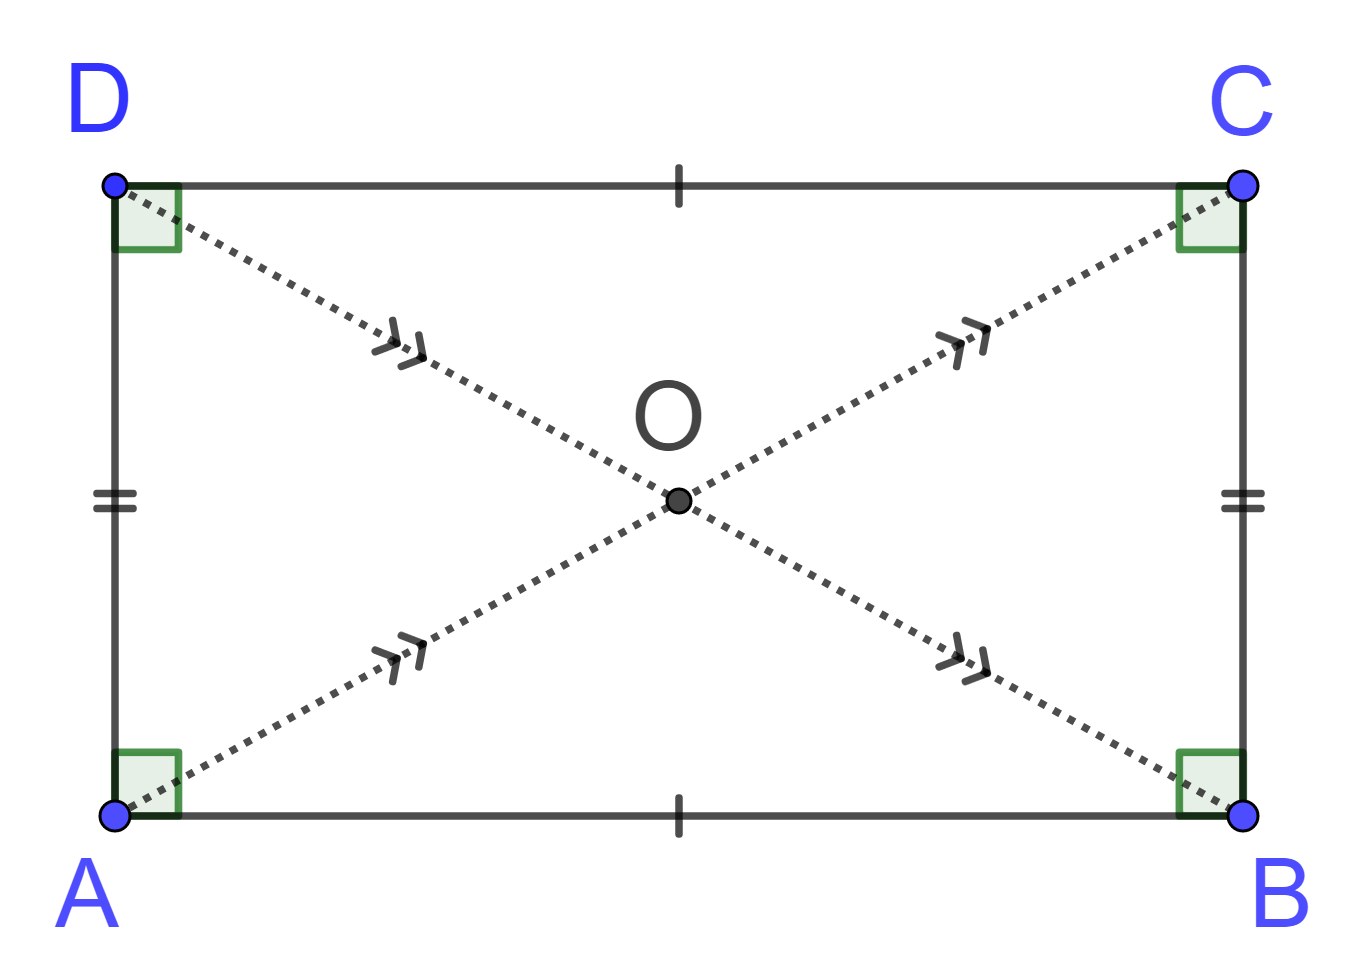
\includegraphics[scale=0.15]{rectangle}
	\end{center}

	ABCD est un rectangle donc :
		\begin{itemize}
			\item $\widehat{ABC} = \widehat{BCD} = \widehat{CDA} = \widehat{DAB} = 90\degree$;
			\item $AC = BD$.
		\end{itemize} 
\end{myex}
		
		
	\subsection{Losange}
		\begin{mydef}
	Un losange est un quadrilatère qui possède \kw{quatre côtés de même longueur}.
\end{mydef}

\begin{myprops}
	\textbf{Si} un quadrilatère est un losange \textbf{alors} 
	\begin{itemize}
		\item ses \kw{quatre cotés} font la \kw{même longueur};
		\item ses \kw{diagonales} ont \kw{perpendiculaires}.
	\end{itemize}
\end{myprops}

\begin{myex}
	\begin{center}
		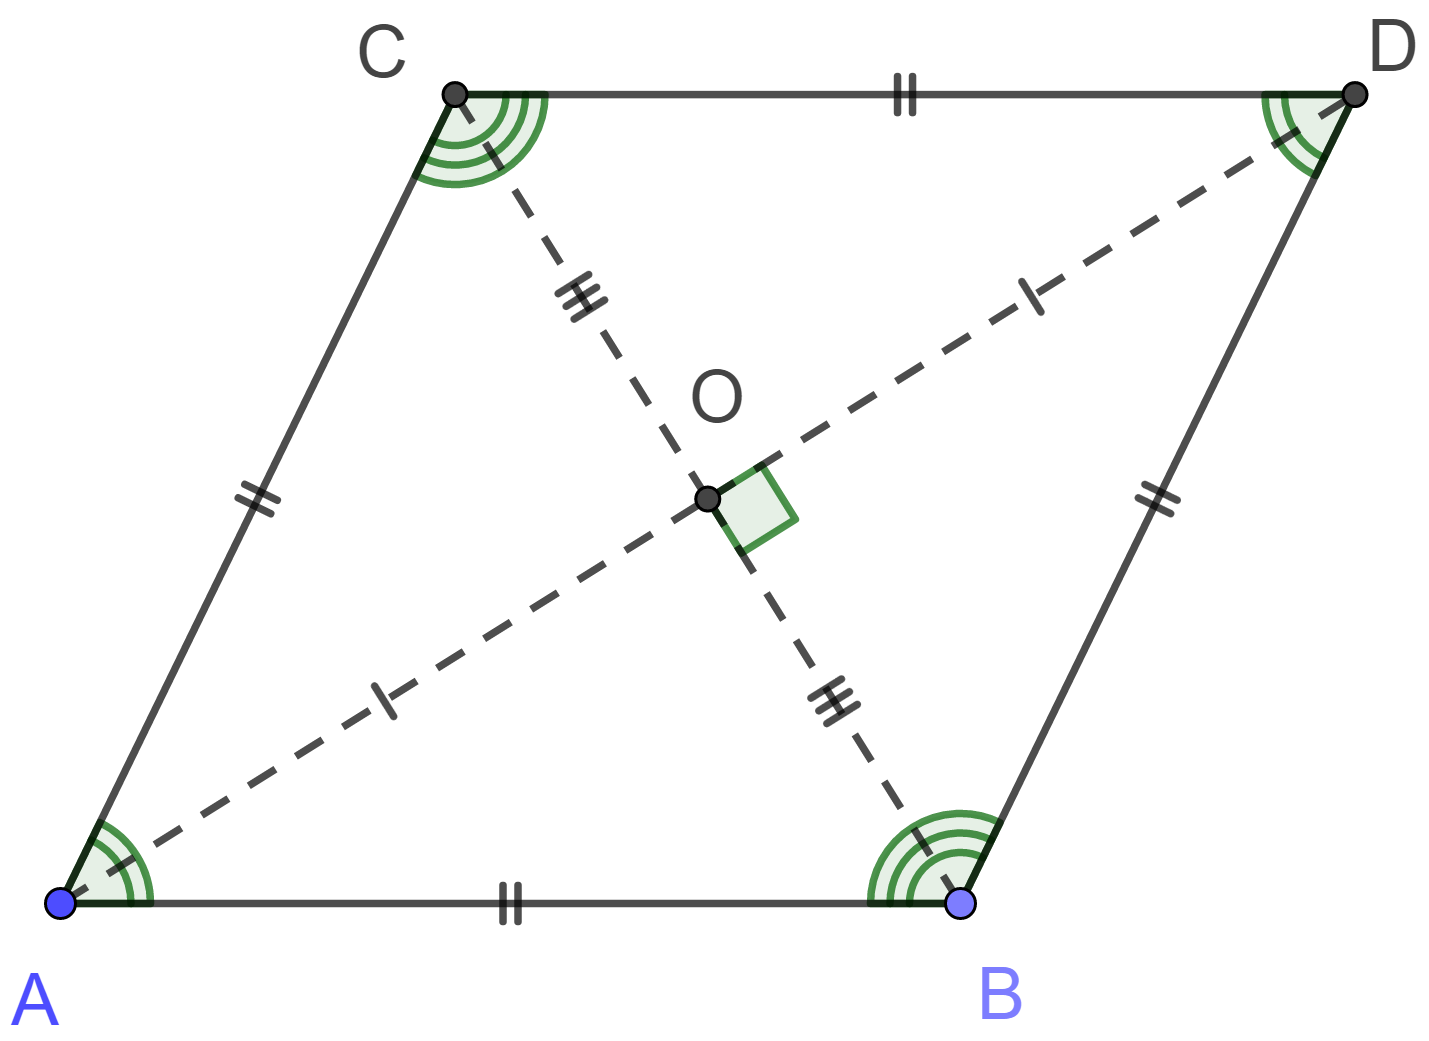
\includegraphics[scale=0.15]{losange}
	\end{center}

	ABCD est un losange donc :
 	\begin{itemize}
 		\item $AB = BC = CD = DA$ ;
 		\item $(AC) \perp (BD)$.
 	\end{itemize}	
\end{myex}
	
	\subsection{Carré}
		\begin{mydef}
	Un carré est un quadrilatère qui possède \kw{quatre angles droits} et \kw{quatre côtés de même longueur}.
\end{mydef}

\begin{myprops}
	\textbf{Si} un quadrilatère est un carré \textbf{alors} 
	\begin{itemize}
		\item ses \kw{quatre cotés} ont la \kw{même longueur};
		\item il a \kw{quatre angles droits};
		\item ses \kw{diagonales} sont \kw{perpendiculaires} et ont la \kw{même longueur}.
	\end{itemize}
\end{myprops}

\begin{myex}
	\begin{center}
		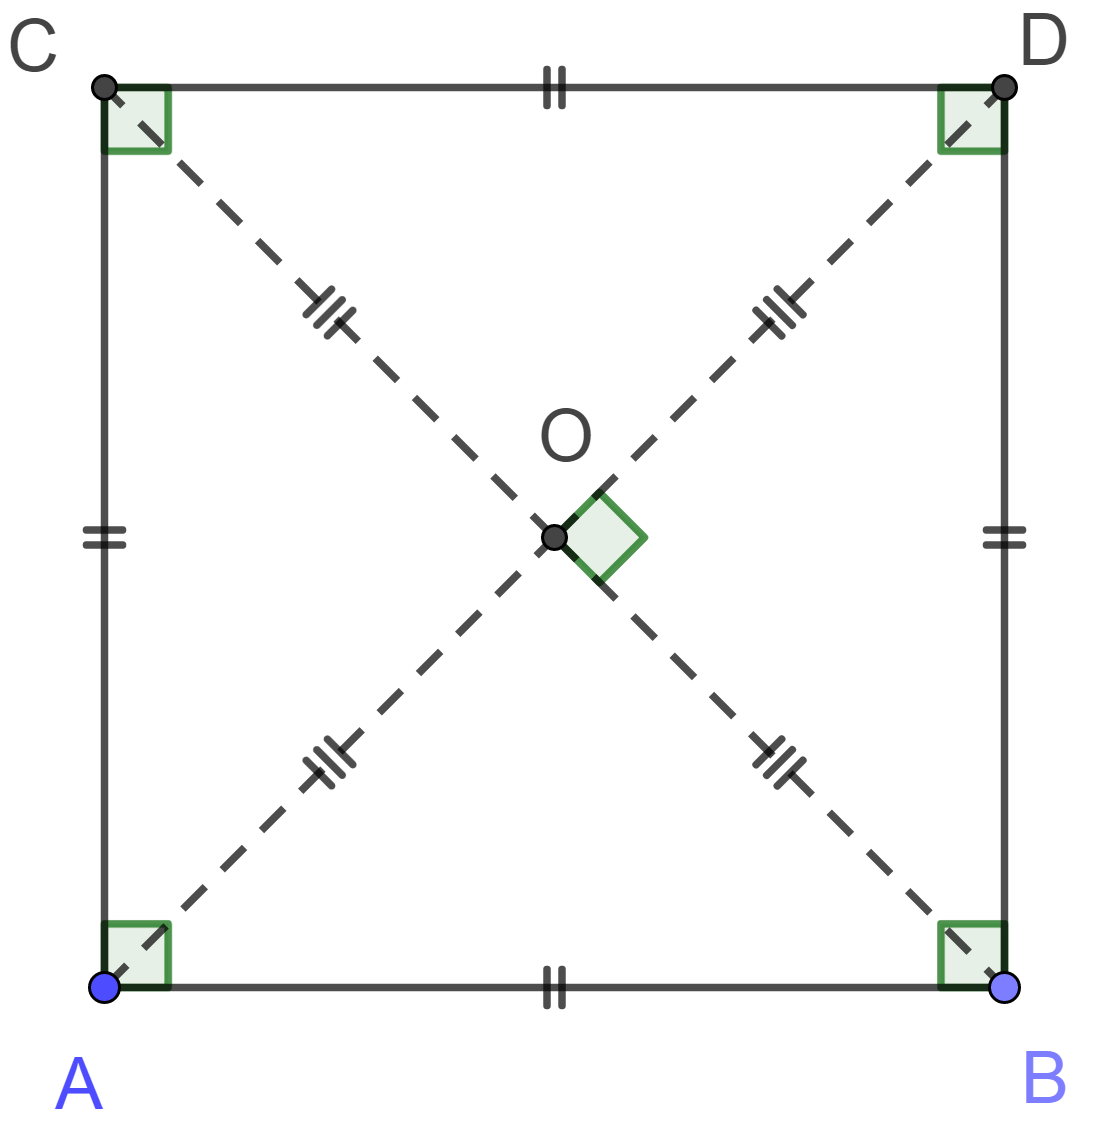
\includegraphics[scale=0.15]{carre}
	\end{center}

	ABCD est un carré donc \begin{itemize}
		\item $AB = BC = CD = DA$;
		\item  $\widehat{ABC} = \widehat{BCD} = \widehat{CDA} = \widehat{DAB} = 90\degree$;
		\item $AC = BD $;
		\item $(AC) \perp (BD)$.
	\end{itemize}
\end{myex}

\newpage
	
\section{Identifier un parallélogramme}	
	\subsection{Du quadrilatère au parallélogramme}

	\begin{myprops}
		\begin{itemize}
			\item \textbf{Si} un quadrilatère a ses \kw{côtés opposés parallèles} \textbf{alors} c'est un parallélogramme.
			\item \textbf{Si} un quadrilatère (non croisé) a ses \kw{côtés opposés de même longueur} \textbf{alors} c'est un parallélogramme.
			\item \textbf{Si} un quadrilatère (non croisé) a \kw{deux côtés opposés parallèles et de même longueur} \textbf{alors} c'est un parallélogramme.
			
			\item \textbf{Si} un quadrilatère a ses \kw{diagonales qui se coupent en leur milieu} \textbf{alors} c'est un parallélogramme.
			
		\end{itemize}
	\end{myprops}

	\begin{myex}
		Déterminer la nature du quadrilatère ABCD sachant que $(AB)//(CD)$.
		
			\begin{center}
				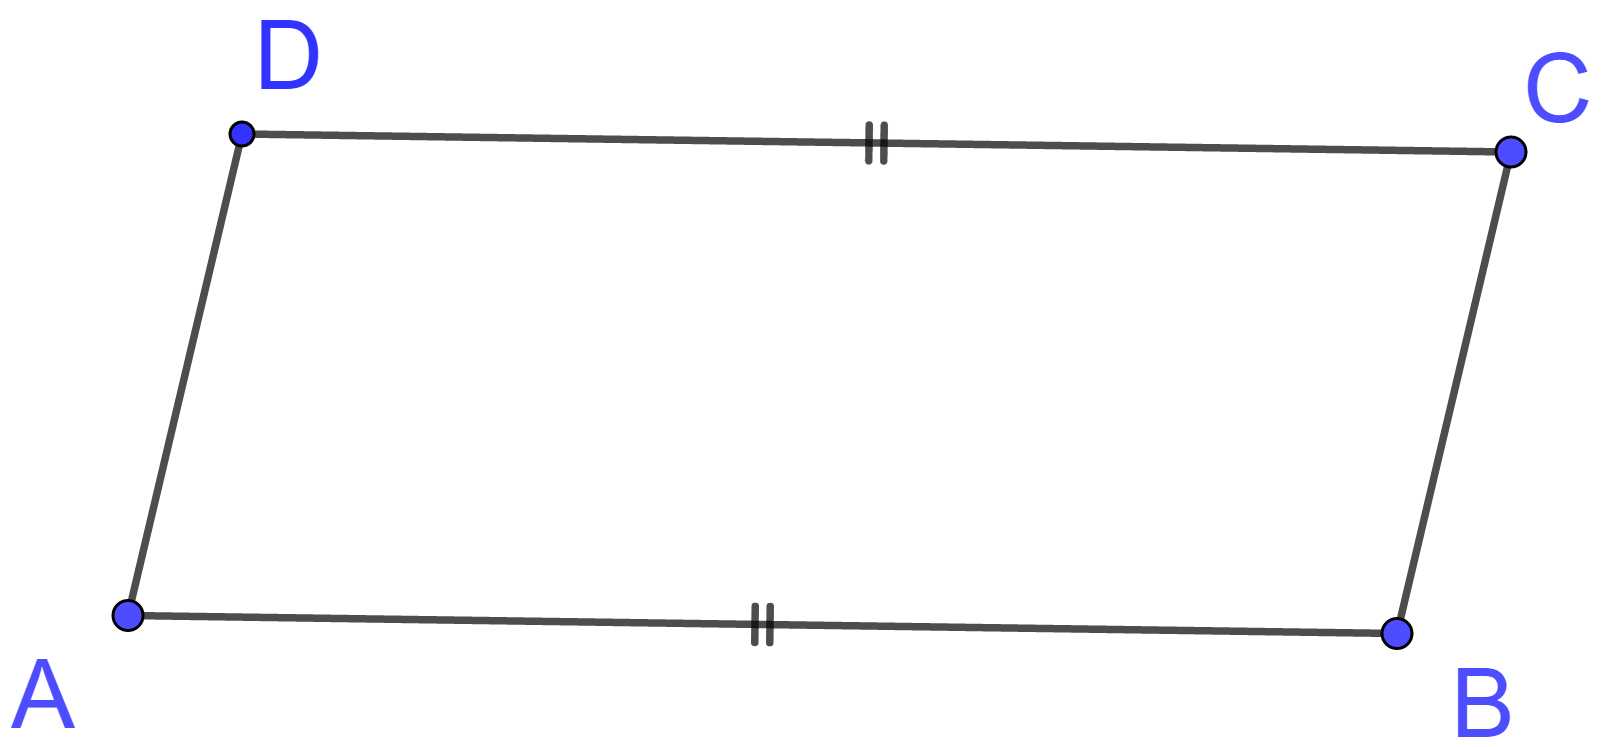
\includegraphics[scale=0.15]{demo1}
			\end{center}
			
			Je sais que $(AB)//(CD)$ et $AB=CD$.
			
			Or si un quadrilatère (non croisé) a deux côtés opposés parallèles et de même longueur alors c'est un parallélogramme.
			
			Donc ABCD est un parallélogramme.
			
		
	\end{myex}


\subsection{Du parallélogramme aux parallélogrammes particuliers}

	\begin{myprop}
		
		\begin{itemize}
			\item \textbf{Si} un parallélogramme a \kw{deux côtés consécutifs perpendiculaires} \textbf{alors} c'est un rectangle.
			\item \textbf{Si} un parallélogramme a \kw{ses diagonales de même longueur} \textbf{alors} c'est un rectangle.
		\end{itemize}
	\end{myprop}


	\begin{myex}
		Déterminer la nature du parallélogramme ABCD.
		
		\begin{center}
			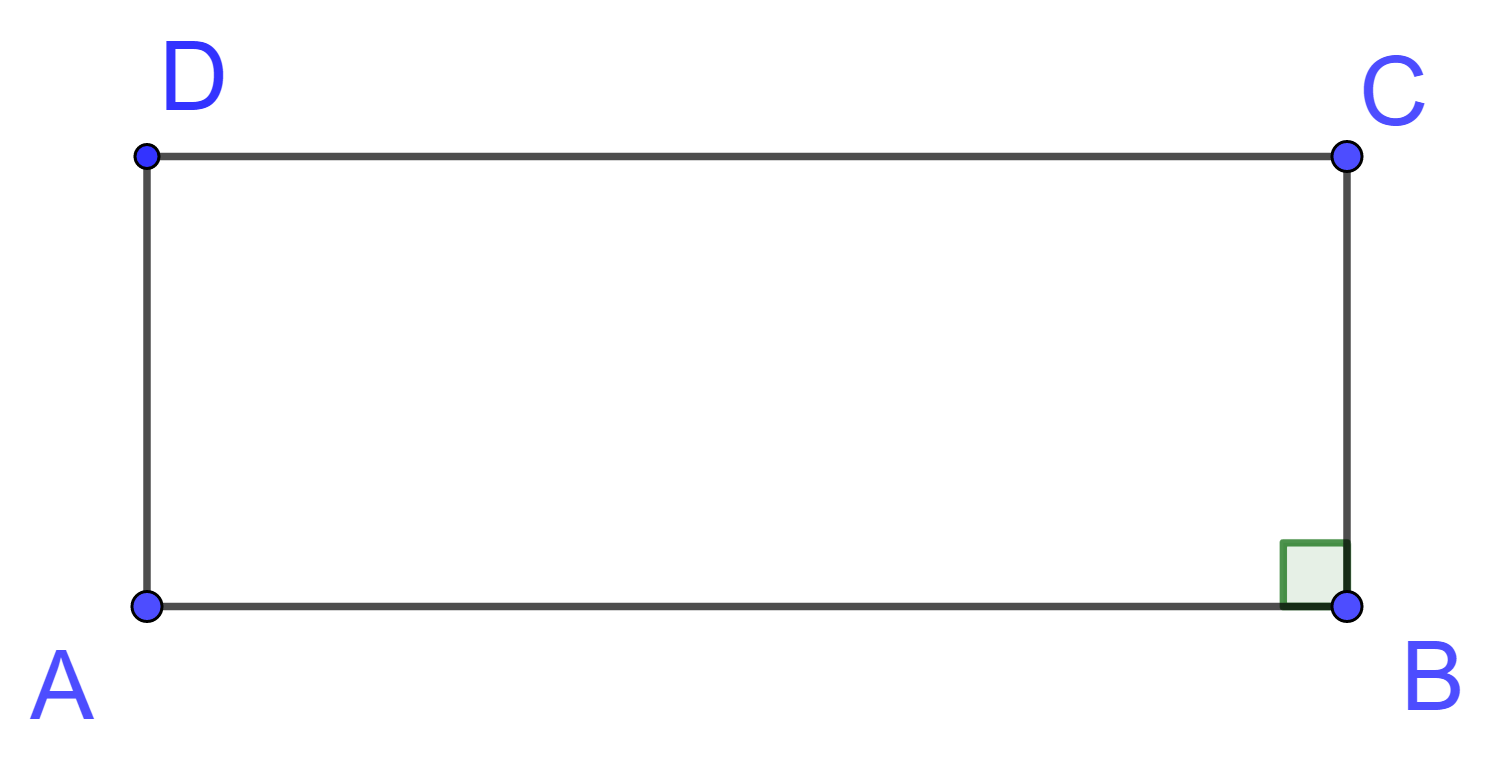
\includegraphics[scale=0.15]{demo2}
		\end{center}
		
		Je sais que ABCD est un parallélogramme et $(AB) \perp (BC)$.
		
		Or si un parallélogramme a deux côtés consécutifs perpendiculaires alors c'est un rectangle.
		
		Donc ABCD est un rectangle.
		
		
	\end{myex}

	\begin{myprops}
		\begin{itemize}
			\item \textbf{Si} un parallélogramme a \kw{deux côtés consécutifs de même longueur} \textbf{alors} c'est un losange.
			\item \textbf{Si} un parallélogramme a \kw{ses diagonales perpendiculaires} \textbf{alors} c'est un losange.
		\end{itemize}
		
	\end{myprops}

	\begin{myex}
		Déterminer la nature du parallélogramme ABCD.
		
		\begin{center}
			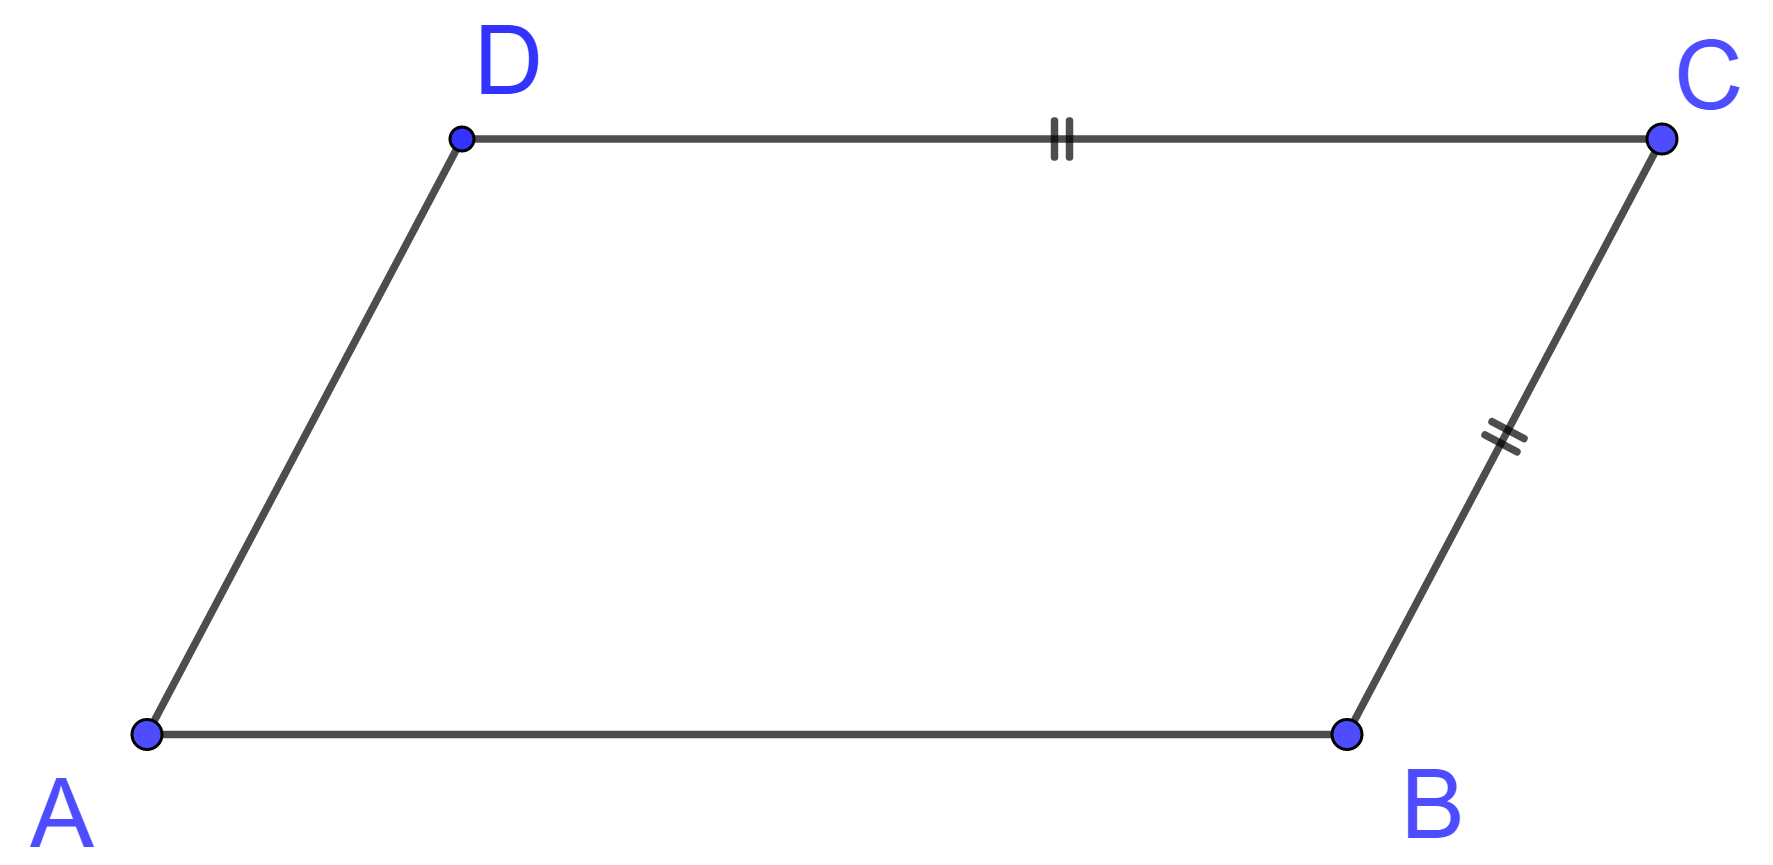
\includegraphics[scale=0.15]{demo3}
		\end{center}
		
		Je sais que ABCD est un parallélogramme et $BC=CD$.
		
		Or si un parallélogramme a deux côtés consécutifs de même longueur alors c'est un losange.
		
		Donc ABCD est un losange.
		
		
	\end{myex}

\newpage

	\begin{myprop}
		\textbf{Si} un quadrilatère est \kw{à la fois un losange et un rectangle} \textbf{alors} c'est un carré.
	\end{myprop}


	
%	\begin{myprop}
%		\begin{itemize}
%			\item \textbf{Si} un parallélogramme a \kw{deux côtés consécutifs de même longueur et perpendiculaires}   \textbf{alors} c'est un carré.
%			\item \textbf{Si} un parallélogramme a \kw{ses diagonales perpendiculaires et de même longueur} \textbf{alors} c'est un losange.
%		\end{itemize}
%	\end{myprop}


	\begin{myex}
		Déterminer la nature du quadrilatère ABCD.
		
		\begin{center}
			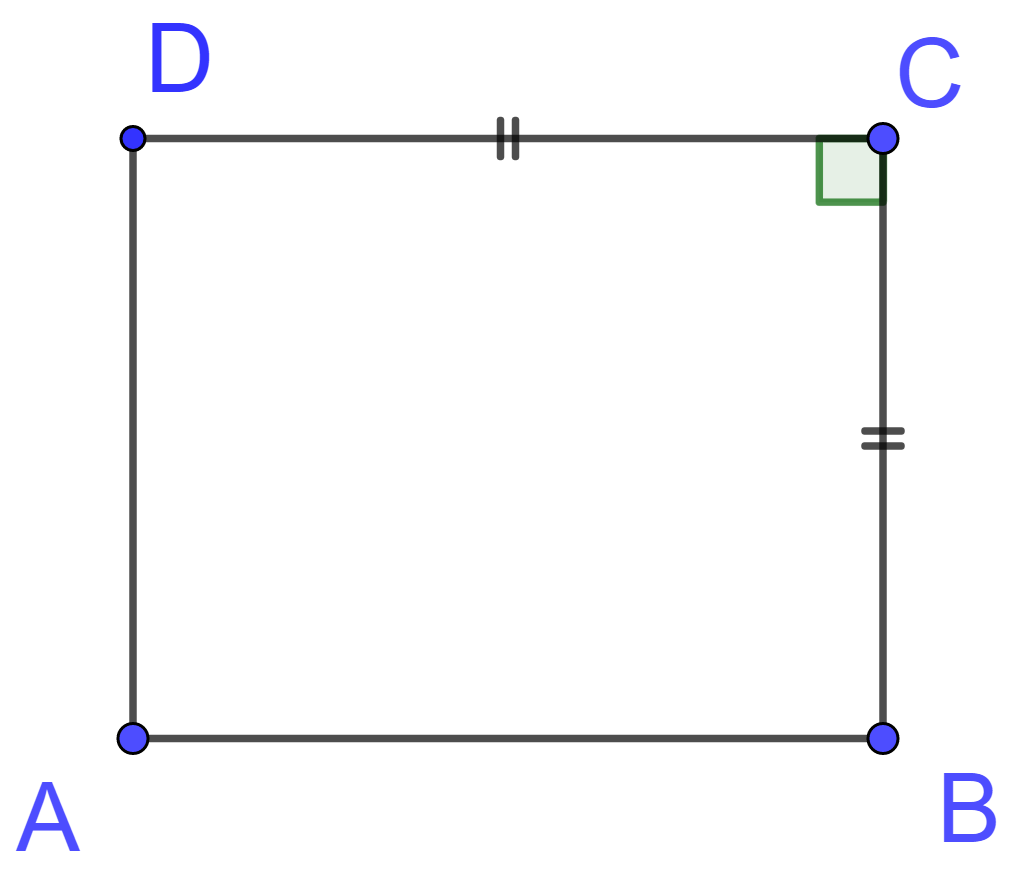
\includegraphics[scale=0.18]{demo4}
		\end{center}
		
		Je sais que ABCD est un parallélogramme et $BC=CD$.
		
		Or si un parallélogramme a deux côtés consécutifs de même longueur alors c'est un losange.
		
		Donc ABCD est un losange.\\
		
		Je sais que ABCD est un parallélogramme et $(BC) \perp (CD)$.
		
		Or si un parallélogramme a deux côtés consécutifs perpendiculaires alors c'est un rectangle.
		
		Donc ABCD est un rectangle.\\
		
		Je sais que ABCD est un losange et ABCD est un rectangle.
		
		Or si un quadrilatère est à la fois un losange et un rectangle alors c'est un carré.
		
		Donc ABCD est un carré.
	\end{myex}
	
	
	


\end{document}

